\newpage
\section{Turing Machine}
%TODO 图 TM?

\subsection{Definition}

\begin{enumerate}
    \item $\leftarrow, \rightarrow$
    \item raed and write
\end{enumerate}

\begin{itemize}
    \item left end symbol $\triangleright$
    \item blank symbol $\sqcup $
\end{itemize}

\begin{definition}
    A Turing machine is a 5-tuple $M=(K, \Sigma, \delta, s, H)$
    \begin{itemize}
        \item $K$: a finite set of states
        \item $\Sigma$: tape alphabet (left end symbol and blank symbol)
        \item $s\in K$: initial state
        \item $H\subseteq K$: a set of halting state
        \item $\delta$: 
    \end{itemize}
    \begin{align*}
        \underbrace{(K-H)}_{\text{\tiny current state}} \times \underbrace{\Sigma}_{\text{\tiny symbol read by the head}} \to \underbrace{K}_{\text{\tiny next state}} \times \underbrace{(\overbrace{\{ \leftarrow, \rightarrow \}}^{\text{\tiny moving}}\cup \overbrace{(\Sigma -\{ \triangleright  \})}^{\text{\tiny writing}})}_{\text{\tiny head action}}
    \end{align*}
    s.t. $\forall q\in K-H$, $\delta(q,\triangleright)=(p, \rightarrow)$ for some $p\in K$
\end{definition}

\begin{definition}[configuration]
    A configuration is a member of 
    \begin{align*}
        K \times \triangleright (\Sigma -\{ \triangleright \})^*\times \left(\{ e \}\cup (\Sigma -\{ \triangleright \})^*(\Sigma -\{ \triangleright, \sqcup\})\right)
    \end{align*}
\end{definition}

\begin{definition}[yield one step]
    \quad 

    $(q_1, \triangleright w_1 \underline{a_1} u_1)\vdash_M (q_2, \triangleright w_2 \underline{a_2} u_2)$ if 
    \begin{enumerate}
        \item writing: $\delta (q_1, a_1)=(q_2,a_2)$, $w_1=w_2$ and $u_1=u_2$
        \item moving left: $\delta(q_1, a)=(q_2,\leftarrow)$, $w_1=w_2a_2$, and $u_2=a_1 u_1$ ($u_2=e$ if $a_1=\sqcup, u_1=e$)
        \item moving right: $\delta(q_1, a)=(q_2,\rightarrow)$, $w_2=w_1a_1$, and $u_1=a_2 u_2$ 
    \end{enumerate}
\end{definition}

\begin{definition}[yields]
    \quad

    $(q_1, \triangleright w_1 \underline{a_1} u_1)\vdash_M^* (q_2, \triangleright w_2 \underline{a_2} u_2)$ if 
    \begin{enumerate}
        \item $(q_1, \triangleright w_1 \underline{a_1} u_1)\vdash_M (q_2, \triangleright w_2 \underline{a_2} u_2)$
        \item $(q_1, \triangleright w_1 \underline{a_1} u_1)\vdash_M \cdots \vdash_M (q_2, \triangleright w_2 \underline{a_2} u_2)$
    \end{enumerate}
\end{definition}

\begin{itemize}
    \item $(q, \triangleright w\underline{a}u)$ is a halting configuration if $q\in H$. 
    \item initial configuration %TODO
\end{itemize}

Fix $\Sigma$
\begin{enumerate}
    \item symbol writing machine $M_a$, $(a\in \Sigma-\{ \triangleright \})$.
    \subitem $M_a=(\{s,h \},\Sigma, \delta, s, \{ h \})$
    \begin{itemize}
        \item $\forall b\in \Sigma-\{\triangleright\}$, $\delta(s,b)=(h,a)$
        \item $\delta(s,\triangleright)=\delta(s,\rightarrow)$
    \end{itemize}
    \item heading moving machine $M_{\rightarrow}$, $M_{\leftarrow}$
    \subitem $M_\leftarrow=(\{s,h \},\Sigma, \delta, s, \{ h \})$
    \begin{itemize}
        \item $\forall b\in \Sigma-\{\triangleright\}$, $\delta(s,b)=(h,\leftarrow)$
        \item $\delta(s,\triangleright)=\delta(s,\rightarrow)$
    \end{itemize}
\end{enumerate}

basic machine: $M_a, M_\leftarrow, M_\rightarrow$, also called $a, L, R$. 

\begin{figure}[!htb]
    \centering
    \begin{tikzpicture}[shorten >=1pt, node distance=2cm, on grid, auto]
        \node[initial] (M_1) {$M_1$};
        \node at (1.2, 0)(M_2) {$M_2$};
        \node at (0, -1.2) (M_3) {$M_3$};
        
        \path [->] (M_1) edge node {$1$} (M_3)
                         edge node {$0$} (M_2)
            ;
    \end{tikzpicture}
    \caption{组合 图灵机}
\end{figure}
\begin{algorithm}[!htb]
    \caption{组合 图灵机}
    \begin{algorithmic}
        \State run $M_1$ until it halts
        \If{the symbol read by head is 0}
            \State run $M_2$
        \ElsIf{the symbol read by head is 1}
            \State run $M_3$
        \Else
            \State halt
        \EndIf
    \end{algorithmic}
\end{algorithm}

\begin{figure}[!htb]
    \centering
    \begin{subfigure}{0.22\textwidth}
        \begin{tikzpicture}[shorten >=1pt, node distance=2cm, on grid, auto]
            \node[initial] (M_1) {$R$};
            \node [right =of M_1] (M_2) {$R$};
            
            \path [->] (M_1) edge node {$\Sigma$} (M_2)
                ;
        \end{tikzpicture}
        \caption{$R^2$}
    \end{subfigure}
    \begin{subfigure}{0.22\textwidth}
        \begin{tikzpicture}[shorten >=1pt, node distance=2cm, on grid, auto]
            \node[initial] (M_1) {$R$};
            \node [right =of M_1] (M_2) {$Ra$};
            
            \path [->] (M_1) edge node {$a\ne \sqcup$} (M_2)
                ;
        \end{tikzpicture}
        \caption{}
    \end{subfigure}

    \begin{subfigure}{0.22\textwidth}
        \begin{tikzpicture}[shorten >=1pt, node distance=2cm, on grid, auto]
            \node[initial] (M_1) {$R$};
            
            \path [->] (M_1) edge [loop right] node {$\overline{\sqcup}$} ()
                ;
        \end{tikzpicture}
        \caption{$R_\sqcup$}
    \end{subfigure}
    \begin{subfigure}{0.22\textwidth}
        \begin{tikzpicture}[shorten >=1pt, node distance=2cm, on grid, auto]
            \node[initial] (M_1) {$L$};
            
            \path [->] (M_1) edge [loop right] node {${\sqcup}$} ()
                ;
        \end{tikzpicture}
        \caption{$L_{\overline{\sqcup}}$}
    \end{subfigure}

    \begin{subfigure}{0.22\textwidth}
        \begin{tikzpicture}[shorten >=1pt, node distance=2cm, on grid, auto]
            \node[initial] (M_1) {$R$};
            
            \path [->] (M_1) edge [loop right] node {${\sqcup}$} ()
                ;
        \end{tikzpicture}
        \caption{$R_{\overline{\sqcup}}$}
    \end{subfigure}
    \begin{subfigure}{0.22\textwidth}
        \begin{tikzpicture}[shorten >=1pt, node distance=2cm, on grid, auto]
            \node[initial] (M_1) {$L$};
            
            \path [->] (M_1) edge [loop right] node {$\overline{\sqcup}$} ()
                ;
        \end{tikzpicture}
        \caption{$L_\sqcup$}
    \end{subfigure}
    \caption{Example}
\end{figure}



Left shifting machine: $S_\leftarrow$. 
$\forall w\in(\Sigma-\{ \triangleright,\sqcup \})^*$, 
\begin{align*}
    \triangleright \sqcup \sqcup w \underline{\sqcup} \to \triangleright \sqcup w \underline{\sqcup} 
\end{align*}
\begin{figure}[!htb]
    \centering
    \begin{tikzpicture}[shorten >=1pt, node distance=2cm, on grid, auto]
        \node [initial] at (0.4, 0) (L_u) {$L_\sqcup$};
        \node at (2,0) (R) {$R$};
        \node at (4,0) (uLaR) {$\sqcup LaR$};
        \node at (2,-1.2) (L) {$L$};

        \path[->] (L_u) edge (R)
                  (R) edge node {$\sqcup$} (L)
                      edge node {$a\ne\sqcup$} (uLaR)
            ;
        \draw [->] (uLaR.east)--(4.8, 0)--(4.8, 0.6)--(2, 0.6)--(R);
    \end{tikzpicture}
    \caption{Left shifting machine: $S_\leftarrow$. }
\end{figure}


\subsubsection{Recognize Language}
\begin{itemize}
    \item input alphabet: $\Sigma_0\subseteq (\Sigma-\{ \triangleright, \sqcup \})$
    \item initial configuration $\{ s, \triangleright\underline{ \sqcup } w \}$
\end{itemize}

\begin{definition}
    $M$ semidecides $L(M)$, called recursively enumerable (递归可枚举)/recognizable
    \begin{align*}
        L(M)=\{ w\in\Sigma_0^*: (s, \triangleright\underline{ \sqcup } w  ) \vdash^* (h,\dots) \text{ for some }h\in H\}
    \end{align*}
\end{definition}
实际上没法用, 因为不保证可接受时间内停机. 

\begin{definition}
    Let $M=(K,\Sigma_0, \Sigma, \delta, s, \{ y,n \})$ be a Turing Machine. We say $M$ decides a language $L\subseteq \Sigma^*$ if 
    \begin{enumerate}
        \item $\forall w\in L$
        \begin{align*}
            (s,  \triangleright\underline{ \sqcup } w)\vdash^*(y,\dots)
        \end{align*}
        $M$ accepts $w$
        \item $\forall w\in \Sigma^*-L$
        \begin{align*}
            (s,  \triangleright\underline{ \sqcup } w)\vdash^*(n,\dots)
        \end{align*}
        $M$ rejects $w$
    \end{enumerate} 

    A language is recursive/decidable if it is decided by some Turing Machine. 
\end{definition}

\begin{theorem}
    If $L$ is recursive, $L$ must is recursively enumerable. 
\end{theorem}
Idea: 构造 n 不停机, y 停机.

\subsection{Compute Function}
\begin{definition}
    $\forall w\in\Sigma_0^*$, if $(s, )\vdash^*(h, \triangleright \underline{\sqcup}y)$ for some $h\in H$ and some $y\in\Sigma^*_0$. 
    \begin{figure}[!htb]
        \centering
        
\includegraphics[width=0.22\textwidth]{pic/TC5/output.png}
        \caption{output}
    \end{figure}
    
    y: output of $M$ on $w$. $y=M(w)$. 

    Let $f:\Sigma^*_0\to \Sigma^*_0$. We say $M$ computes $f$ if 
    \begin{align*}
        \forall w\in \Sigma^*_0, M(w)=f(w)
    \end{align*}
    $f$ is called recursive/computable
\end{definition}

e.g. $\{ a^nb^nc^n:n\ge0 \}$ is recursive. 
%TODO 有问题, 需要修正, 可以接受 abcabc 之类的串
\begin{figure}[!htb]
    \centering
    \begin{tikzpicture}[shorten >=1pt, node distance=2cm, on grid, auto]
        \tikzmath{
            \step=1.6;
        } 
        \node [initial] (R) {$R$};
        \node at (\step, 0) (xR1) {$\times R$};
        \node at (2*\step, 0) (xR2) {$\times R$};
        \node at (3*\step, 0) (xlu) {$\times L\sqcup$};
        \node at (0    , -\step) (y) {$y$};
        \node at (\step, -\step) (n) {$n$};

        \path [->]  (R) edge node {$a$} (xR1)
                        edge node {$\sqcup$} (y)
                        edge node {$b,c$} (n)
                        edge [in=30, out=60, loop] node  [above] {$\times$} ()
                    (xR1) edge node {$b$} (xR2)
                        edge node {$c$} (n)
                        edge [loop above] node [above] {$a, \times$} ()
                    (xR2) edge node {$c$} (xlu)
                        edge node {$a$} (n)
                        edge [loop above] node [above] {$b, \times$} ()
                ;
        \draw [->] (xlu)--(3*\step, \step)--(0, \step)--(R);
    \end{tikzpicture}
    \caption{$\{ a^nb^nc^n:n\ge0 \}$}
\end{figure}

\subsection{Extensions of Turing machines}
\subsubsection{Multiple tape TM}
\begin{align*}
    \delta: (K-H)\times \Sigma^k \to K\times (\Sigma \cup \{ \leftarrow, \rightarrow \})^k
\end{align*}

\begin{figure}[!htb]
    \centering
    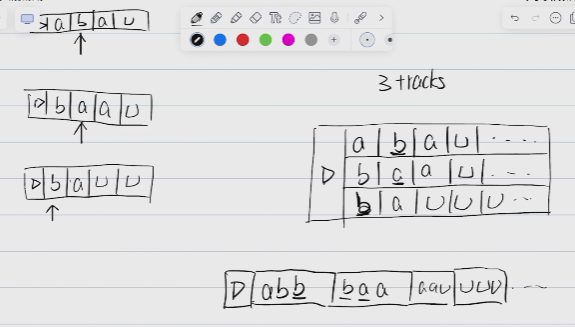
\includegraphics[width=0.309\textwidth]{pic/TC5/idea-mTM.png}
    \caption{Multiple tape TM}
\end{figure}

Idea: 以三带为例, 将一条纸带分为三个 tracks, 也可以等价于把纸带拉平, 其 symbol 长度为 3. 

\subsubsection{Two-way Infinite Tape}
\begin{figure}[!htb]
    \centering
    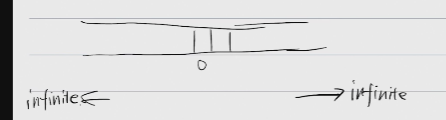
\includegraphics[width=0.309\textwidth]{pic/TC5/twi.png}
    \caption{Two-way Infinite Tape}
\end{figure}

向两侧无限延申. 

可以先使用双带模拟, 然后用标准 TM 模拟双带.

\subsubsection{Multiple Heads}
\begin{figure}[!htb]
    \centering
    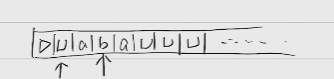
\includegraphics[width=0.309\textwidth]{pic/TC5/mh.png}
    \caption{Multiple Heads}
\end{figure}

一个纸带但多个读写头. 

用下划线标记这 $k$ 个读写头, 先找到 $k$ 个下划线位置, 然后做操作. 

\subsubsection{Two-Dimensional Tape}
\begin{figure}[!htb]
    \centering
    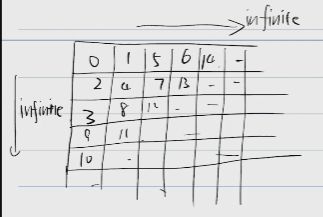
\includegraphics[width=0.309\textwidth]{pic/TC5/tdt.png}
    \caption{Two-Dimensional Tape}
\end{figure}

二维纸带. 

将所有格子做编号, 然后拉平. 

\subsubsection{Random Access TM}
head 可以跳格子. 

把跳拆开成单步走即可. 

\subsection{Non-deterministic TM}
\begin{definition}
    A non-deterministic Turing Machine is 5-tuple $M=(K, \Sigma, \Delta, s, H)$
    \begin{itemize}
        \item $K$
        \item $\Sigma$
        \item $s$
        \item $H$
        \item $\Delta$: a finite set of 
        \begin{align*}
            ((K-H)\times \Sigma)\times (K\times \Sigma \cup \{ \leftarrow , \rightarrow \})
        \end{align*}
    \end{itemize}
\end{definition}
可以看作是一颗树. 

Also can define configuration and $\vdash_M, \vdash_M^*, \vdash_M^N$ (走 $N$ 步). 

\begin{definition}
    A NTM $M$ with input alphabet $\Sigma_0$, semidecides $L\subseteq \Sigma_0^*$, if $\forall w \in \Sigma_0^*$, $w\in L$ iff $(S, \triangleright \sqcup w)\vdash^*_M (h,\dots)$ for some $h$. 
\end{definition}

\begin{definition}
    Let $M=(K, \Sigma, \Delta, s, \{ y,n \})$ be a NTM with input alphabet $\sigma_0$. $M$ decides a language $L\in \Sigma_0^*$ if 
    \begin{enumerate}
        \item there is a constant $N$ (independent of the $M$), $\forall w\in \Sigma_0^*$, there is no configuration $C$, satifiy $(s,\triangleright \underline{\sqcup} w)\vdash_M^N C$. (要求每条分支在 $N$ 步内停止)
        \item $w\in L$ iff $(s,\triangleright \underline{\sqcup} w)\vdash_M^*(y,\dots)$
    \end{enumerate}
\end{definition}
即 NTM 树高有限, 且
\begin{itemize}
    \item if $w\in L$, some branch accepts $w$
    \item if $w\notin L$, every branch rejects $w$
\end{itemize}

e.g. Let $C=\{ 100, 110, 1000, \dots \}$ (所有合数二进制编码集合) 

Idea: 猜其两个分解 $p,q$, if $p\times q=w$ accepts it, else rejects it. 

\begin{theorem}
    Every NTM can be simulated by a DTM. 
\end{theorem}
\begin{proof}(sketch)以 semidecides 为例. 

    a NTM semidecides $L$ $\to$ a DTM semidecides $L$. 

    3-tape DTM to simulate NTM (using BFS) 
    \begin{itemize}
        \item store the input $w$
        \item simulate NTM
        \item enumerate hints
    \end{itemize}
\end{proof}


\begin{table}[!htb]
    \centering
    \caption*{Church-Turing Thesis}
    \begin{tabular}{ccc}
        Intuition of algorithm & equals & \begin{tabular}[c]{@{}c@{}}Turing machines that\\ halt on every input\end{tabular} \\
        solve                  &        & decide                                                                             \\
        decision porblem       & equals & language                                                                          
    \end{tabular}
\end{table}

Intuition of algorithm $\iff$ TM that halt of every input


Description of TM
\begin{enumerate}
    \item formal definition: $M=(K,\Sigma, \delta, s, H)$
    \item Implement-level desc: diagram
    \item high-level: ``pseudo code''
\end{enumerate}

Fact:
\begin{enumerate}
    \item Any finite set can encoded. 
    \item Any finite collection of finite sets can be encoded
\end{enumerate}
Object $O$ $\to$ $''O''$ (用双引号表示 encode)% 数学模式中 的 ``''

\subsection{Decidable Problem}
\begin{enumerate}
    \item [$R_1$] $A_{DFA}=\{ ''D''\ ''w'': D \text{ is a DFA that accepts }w \}$. 
    \subitem $M_{R_1}=$ on input $''D''\ ''w''$.

    \begin{algorithm}[!htb]
        \caption{$R_1$}
        \begin{algorithmic}
            \State run $D$ on $w$.
            \If{$D$ accepts $w$}
                \State accepts $''D''\ ''w''$
            \Else
                \State rejects $''D''\ ''w''$
            \EndIf
        \end{algorithmic}
    \end{algorithm}
    \item [$R_2$] $A_{NFA}=\{ ''N''\ ''w'': N \text{ is a NFA that accepts }w \}$
    \subitem $M_{R_2}=$ on input $''N''\ ''w''$.
    \begin{algorithm}[H]
        \caption{$R_2$}
        \begin{algorithmic}
            \State N $\to$ equivalent DFA $D$
            \State run $M_{R_1}$ on $''D''\ ''w''$
            \State output the result of $M_{R_1}$
        \end{algorithmic}
    \end{algorithm}
    a reduction(归约) from $A_{NFA}$ to $A_{DFA}$. 将左输入映射为右输入, 保证映射前后答案一致. 
    \item [$R_3$] $A_{REX}=\{ ''R''\ ''w'': R $ is a regular expression with $w\in L(R)  \}$
    \subitem $M_{R_3}=$ on input $''R''\ ''w''$.
    \begin{algorithm}[H]
        \caption{$R_3$}
        \begin{algorithmic}
            \State R $\to$ an equivalent NFA $N$
            \State run $M_{R_2}$ on $''N''\ ''w''$
            \State output the result of $M_{R_2}$
        \end{algorithmic}
    \end{algorithm}
    \item [$R_4$] $E_{DFA}=\{ ''D'': D \text{ is a DFA and }L(D)=\emptyset \}$
    \subitem $M_{R_4}=$ on input $''D''$
    \begin{algorithm}[H]
        \caption{$R_4$}
        \begin{algorithmic}
            \If{$D$ has no finial state}
                \State accepts
            \Else
                \State run DFS on BFS starting with the initial state on the diagram
                \If{$\exists$ path from $s$ to finial}
                    \State reject
                \Else
                    \State accept
                \EndIf
            \EndIf
        \end{algorithmic}
    \end{algorithm}
    \item [$R_5$] $EQ_{DFA}=\{ ''D_1''\ ''D_2'': D_1$ and $D_2$ are DFAs with $L(D_1)=L(D_2) \}$
    \begin{definition}[symmetric difference]
        \begin{align*}
            A \oplus B = \{ x\in A\cup B \cap x \notin A\cap B \}
        \end{align*}
        \begin{align*}
            A=B &\iff A\oplus B=\emptyset\\
            A\oplus B&=A\cup B-A\cap B\\
            &= (A\cup B)\cap (\overline{A\cap B})\\
            &=(A\cup B)\cap (\overline{A}\cup \overline{B})
        \end{align*}
    \end{definition}
    \subitem $M_{R_5}=$ on input $''D_1''\ ''D_2''$

    \begin{algorithm}[H]
        \caption{$R_5$}
        \begin{algorithmic}
            \State construct $D_3$ with $L(D_3)=L(D_1)\oplus L(D_2)$
            \State run $M_{R_4}$ on $''D_3''$
            \State output the result of $M_{R_4}$
        \end{algorithmic}
    \end{algorithm}
\end{enumerate}

